In \secref{prior_perturbations} we considered a multiplicative perturbations
of the form \eqref{phi_perturbation} with the $\norminf{\cdot}$ norm.  In
this section we consider other norms, illustrating that other choices
have problems with KL divergence.

First, we recall what we hope to get from our linear approximation.  We wish to
approximation $\etaopt(\phi)$ using the linear approximation $\etalin(\phi)$
evaluated at $\phiz$, hoping that the error $\norm{\etaopt(\phi) -
\etalin(\phi)}_2$ is small whenever the $\norm{\phi}$ is small (for some choice
of $\norm{\cdot}$).  A bare minimum for such a local approximation to work is
for $\phi \mapsto \etaopt(\phi)$ to be continuous, so that, for any
$\phi$,
%
\begin{align*}
%
\lim_{t \rightarrow 0} \norm{\etaopt(t \phi) - \etaopt}_2 = 0.
%
\end{align*}
%
By this reasoning, however, $\etaopt$ itself is a ``good'' approximation to
$\etaopt(\phi)$ when $\norm{\phi}$ is small---when $\phi$ is small, by
continuity we can simply say that nothing has changed and be reasonably correct.
From our linear approximation, we expect another order of accuracy, namely that
%
\begin{align*}
%
\lim_{t \rightarrow 0} \frac{\norm{\etaopt(t \phi) - \etalin(t\phi)}_2}{t} = 0.
%
\end{align*}
%
That is, we expect an extra order of accuracy from our linear approximation
in $\norm{\phi}$.

The preceding display is enough if we have a fixed $\phi$ in mind.  However, if
we want to search over a larger set of candidate $\phi$, we want the derivative
to provide a {\em uniformly good approximation} to $\etaopt(\phi)$ amonst some
set of $\phi$, say, all bounded $\phi: \norm{\phi} \le 1$.  One way of
formalizing the notion of ``uniformaly good approximation'' follows.

%%%%%%%%%%%%%%%%%%%%%%%%%%%%%%%%%%%%%%%%%%%%%%%%%%%%%%%%%%%%%%%%%%%%%%%%%%%
%%%%%%%%%%%%%%%%%%%%%%%%%%%%%%%%%%%%%%%%%%%%%%%%%%%%%%%%%%%%%%%%%%%%%%%%%%%
\begin{defn}\deflabel{diffable_classes}
    (\citep[Definition 4.5]{zeidler:2013:functional})
%
Let $B_1$ and $B_2$ denote Banach spaces, and let $\ball_1 \subseteq B_1$ define
an open neighborhood of $\phi_0 \in B_1$.  Fix a function $f: \ball_1
\mapsto B_2$.

The function $f$ is {\em directionally differentiable} (also known as a Gateaux
differentiable) if there exists a bounded linear functional $f^{\mathrm{lin}}:
B_1 \mapsto B_2$ such that
%
\begin{align*}
%
\textrm{For any }\phi: \norm{\phi - \phi_0} = 1\textrm{, }
\lim_{t \rightarrow 0}
    \frac{f(\phi) - f(\phi_0) -
          f^{\mathrm{lin}}(t (\phi - \phi_0) )
         }{t} \rightarrow 0.
%
\end{align*}
%

Similarly, the function $f$ is {\em boundedly differentiable} (also known as
Fr{\'echet} differentiable) at $\phi_0$ if
%
\begin{align*}
%
\lim_{t \rightarrow 0}
    \sup_{\phi: \norm{\phi - \phi_0} = 1}
    \frac{f(\phi) - f(\phi_0) -
          f^{\mathrm{lin}}(t (\phi - \phi_0))
         }{t} \rightarrow 0.
%
\end{align*}
%
\end{defn}
%%%%%%%%%%%%%%%%%%%%%%%%%%%%%%%%%%%%%%%%%%%%%%%%%%%%%%%%%%%%%%%%%%%%%%%%%%%

Note that we used the same notation $f^{\mathrm{lin}}$ for both derivatives in
\defref{diffable_classes}.  In fact, if a function is compactly differentiable
then the two derivatives must coincide \citep[Proposition
4.8]{zeidler:2013:functional}, which justifies our presumptuous notation.

The difference between bounded and directional differentiability is whether the
linear approximation holds uniformly in $\phi$.  It is possible for functions to
be directionally but not boundedly differentiable even in $\mathbb{R}^2$, as the
following example demonstrates.

%%%%%%%%%%%%%%%%%%%%%%%%%%%%%%%%%%%%%%%%%%%%%%%%%%%%%%%%%%%%%%%%%%%%%%%%%
%%%%%%%%%%%%%%%%%%%%%%%%%%%%%%%%%%%%%%%%%%%%%%%%%%%%%%%%%%%%%%%%%%%%%%%%%
\begin{ex}\exlabel{r2_pathological}
%
Consider $(x_1, x_2) \in \mathbb{R}^2$ and the polar coordinates $r :=
\sqrt{x_1^2 + x_2^2}$ and $\theta := \arctan(x_2 / x_1)$.  Let $\{\pi k: k \in
\mathbb{Z} \}$ denote integer multiples of $\pi$.  Define
%
\begin{align*}
%
f(r, \theta) := \begin{cases}
\frac{\left(\frac{r}{| \sin \theta |}\right)^2}
     {1 + \left(\frac{r}{| \sin \theta |}\right)^2}
    & \textrm{when } \theta \notin \{\pi k: k \in \mathbb{Z}\}
    \textrm{ and } r > 0 \\
0. & \textrm{when } \theta \in \{\pi k: k \in \mathbb{Z}
    \} \textrm{ or }r = 0
%
\end{cases}
%
\end{align*}
%
%%%%%%%%%%%%%%%%%%%%%%%%%%%%%%%%%%%%%%%%%%%%%%%%%%%%%%%%%%%%%%%%%%%%%%%%%
%%%%%%%%%%%%%%%%%%%%%%%%%%%%%%%%%%%%%%%%%%%%%%%%%%%%%%%%%%%%%%%%%%%%%%%%%
\begin{figure}[h!]

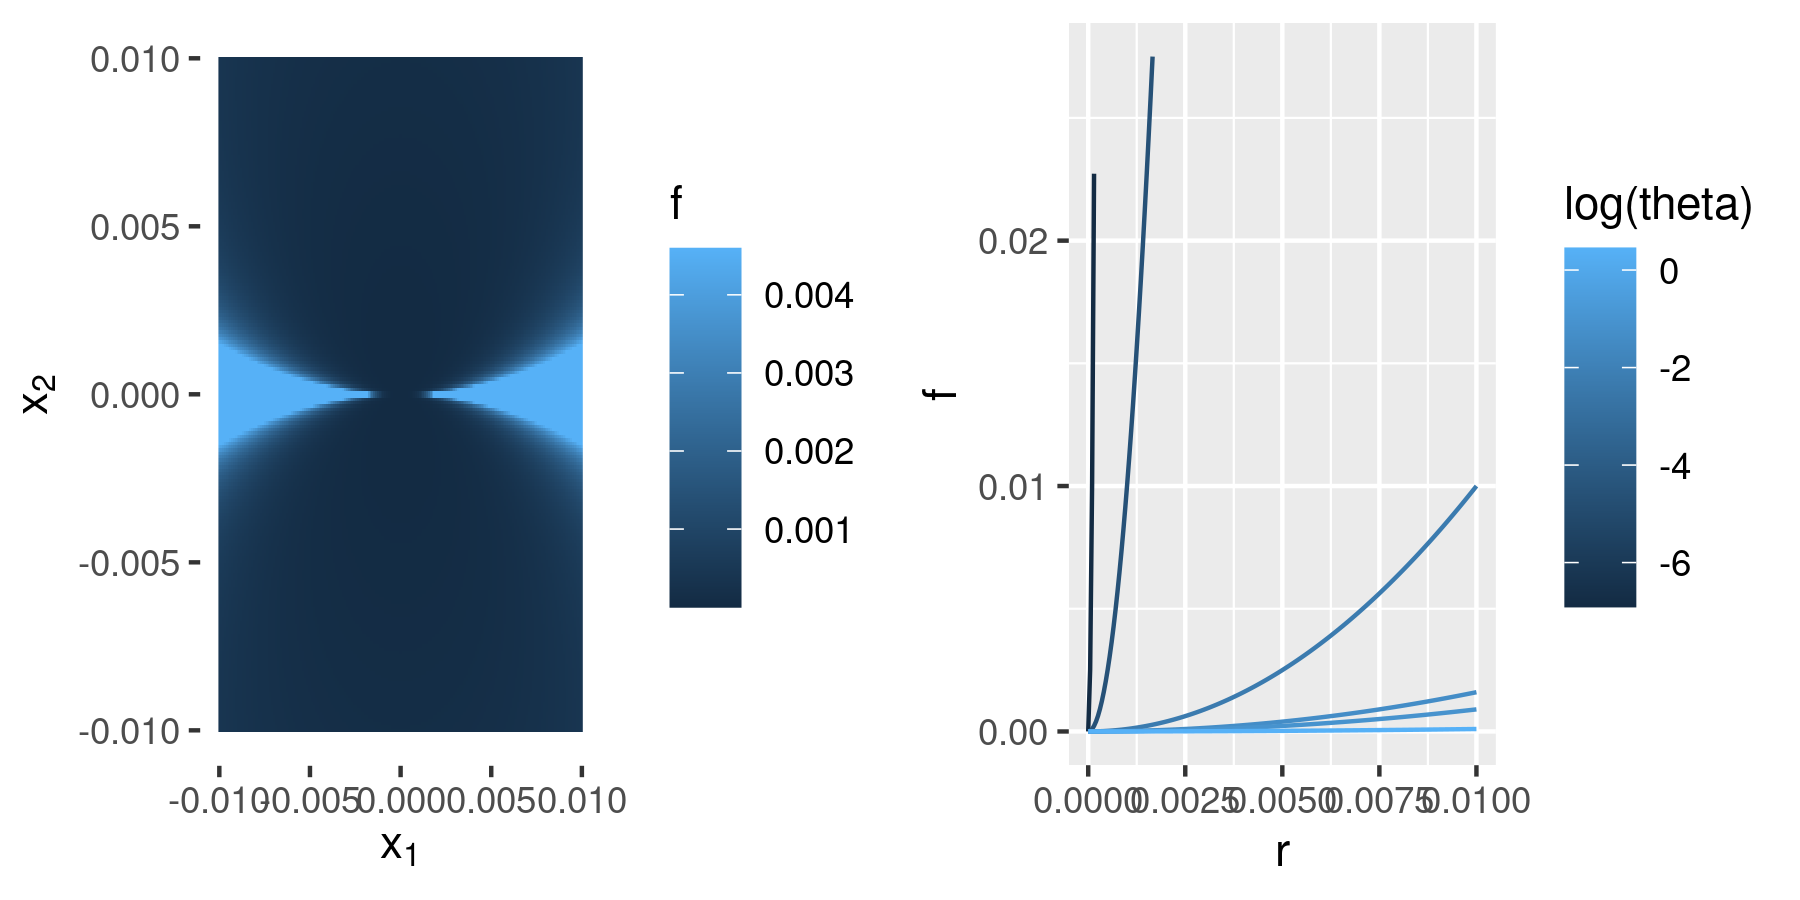
\includegraphics[width=0.980\linewidth,height=0.490\linewidth]{static_images/pathological_r2_example.png}
\caption{A plot of $f(x_1, x_2)$ from \exref{r2_pathological}.}
\figlabel{r2_pathological}
\centering
\end{figure}
%%%%%%%%%%%%%%%%%%%%%%%%%%%%%%%%%%%%%%%%%%%%%%%%%%%%%%%%%%%%%%%%%%%%%%%%%
%
\Figref{r2_pathological} contains a plot of $f(r, \theta)$, both over
$\mathbb{R}^2$ and along paths for particular choices of $\theta$.

Then $f$ has a directional derivative in every direction, but is not Fr{\'e}chet
differentiable. By ordinary calculus, for any $\theta$, $\fracat{\partial f(r,
\theta)}{\partial r}{r=0} = 0$, so the linear approximation to $f(r, \theta)$ at
$r=0$ is identically zero.  However, for any $r$, there exists a $\theta(r)$
such that $r / |\sin(\theta(r))| = 1$.  For such a choice of $\theta(r)$, the
error in the linear approximation is $f(r, \theta(r)) - 0 = 1/2$, which does not
go to zero as $r \rightarrow 0$.

\end{ex}
%%%%%%%%%%%%%%%%%%%%%%%%%%%%%%%%%%%%%%%%%%%%%%%%%%%%%%%%%%%%%%%%%%%%%%%%%

Note that the second derivative in a particular direction is given by
$\fracat{\partial^2 f(r, \theta)}{\partial r^2}{r=0} = \frac{1}{2 |\sin
\theta|}$, which can be made arbitrarily large by taking $\theta$ close to $0$
or to $\pi$.  We could modify $f(r, \theta)$ to be Fr{\'e}chet differentiable
by smoothly ``capping'' $1 / |\sin \theta|$ at some arbitrarily large value.
However, the ability to meaningfully extrapolate $f(r, \theta)$ in the direction
of a very large but finite second derivative will still be extremely limited. In
this sense, Fr{\'e}chet differentiability is a weak necessary but not sufficient
requirement if we are interested in extrapolating using linear approximations.



%%%%%%%%%%%%%%%%%%%%%%%%%%%%%%%%%%%%%%%%%%%%%%%%%%%%%%%%%%%%%%%%%%%%%%%%%
%%%%%%%%%%%%%%%%%%%%%%%%%%%%%%%%%%%%%%%%%%%%%%%%%%%%%%%%%%%%%%%%%%%%%%%%%
\begin{ex}\exlabel{r2_pathological_v2}
%
In the context of \exref{r2_pathological}, fix some $0 < M < \infty$,
and define
%
\begin{align*}
%
\tilde{f}(r, \theta) := \begin{cases}
    f(r, \theta) & \textrm{when }\frac{1}{\abs{\sin(\theta)}} \le M \\
    0. & \textrm{when }\frac{1}{\abs{\sin(\theta)}} > M.
%
\end{cases}
%
\end{align*}
%
Then $\tilde{f}$ is continuous and Fr{\'e}chet differentiable at $r=0$. In this
case, for any $r$, $\sup_{\theta} r / |\sin(\theta(r))| = r / M$, so  both
$\lim_{r \rightarrow 0} \tilde{f}(r, \theta) \le \lim_{r \rightarrow 0} r^2 /
M^2 = 0$ and $\lim_{r \rightarrow 0} \tilde{f}(r, \theta) / r \le \lim_{r
\rightarrow 0}  r / M^2 = 0$.

However, in the direction $\theta = \sin^{-1}(1 / M)$, the error of the linear
extrapolation to any $r_0$ is still $\tilde{f}(r, \theta) - 0 = M r_0^2$. Since
Fr{\'e}chet differentiability requires only $M < \infty$, the extraplation error
can be arbitrarily large for Fr{\'e}chet differentiable functions.

\end{ex}
%%%%%%%%%%%%%%%%%%%%%%%%%%%%%%%%%%%%%%%%%%%%%%%%%%%%%%%%%%%%%%%%%%%%%%%%%


\Exref{r2_pathological} is neither Fr{\'e}chet differentiable nor continuous,
whereas \exref{r2_pathological} is both Fr{\'e}chet differentiable and
continuous.  It turns out that, even in $\mathbb{R}^2$, it is possible for a function
to be ....

Note also that $f(r, \theta)$ is disccontinuous at $r=0$.  It turns out that
this is not essential to the example; see \citet[Example
1.9]{averbukh:1967:theory} for an (only slightly more complicated) example of a
function on $\mathbb{R}^2$ that is continuous and directionally differentiable
but not Fr{\'e}chet differentiable at $r=0$.  Hence continuity does not imply
Fr{\'e}chet differentiability.  However, the converse is true: Fr{\'e}chet
differentiability implies continuity.



A similar example that is more directly relevant is the following.

%%%%%%%%%%%%%%%%%%%%%%%%%%%%%%%%%%%%%%%%%%%%%%%%%%%%%%%%%%%%%%%%%%%%%%%%%
%%%%%%%%%%%%%%%%%%%%%%%%%%%%%%%%%%%%%%%%%%%%%%%%%%%%%%%%%%%%%%%%%%%%%%%%%
\begin{ex}

TODO: make this a lemma.  Then, by saying that \assuref{dist_fun_nice}
holds with $\int M_\psi(\zeta)^{1/q} d\zeta < \infty$ for $1 \le q < \infty$,
I think you will get existence of the $L_p$ derivatives.

Let $\q(\zeta)$ be a density relative to the Lebesge measure on $[0,1]$ such
that $\int \q(\zeta)^p d\zeta < \infty$ for all $1 \le p < \infty$. (Bounded
densities or the Beta distribution are examples.) Define $f: \lp{p} \mapsto
\mathbb{R}$ with $1 \le p < \infty$ as follows:
%
\begin{align*}
%
f(\phi) :=
\begin{cases}
    %
    \expect{\q(\zeta)}{\log \left(1 + \phi(\zeta)\right)} &
    \textrm{when }\phi(\zeta) > -1\textrm{ almost surely} \\
    %
    0 & \textrm{otherwise}.
%
\end{cases}
%
\end{align*}
%
Then, at $\phiz$,  $f(\phi)$ has a directional derivative for every $\phi$, but
is discontinous in $\norm{\cdot}_p$ and so not Fr{\'e}chet differentiable, as
we now show.

For any $0 < \epsilon < 1$, let $S_\epsilon \subset [0, 1]$ be a measurable set
with Lebesgue measure $\epsilon$ and probability at least $\epsilon$ under
$\q(\zeta)$ (such a set must exist because $\int_0^1 \q(\zeta) d\zeta = 1$). For
$\delta > 0$ let
%
\begin{align*}
%
\phi(\zeta; \epsilon, \delta) :=
\begin{cases}
    %
    \delta - 1      & \textrm{ for }\zeta\in S_\epsilon \\
    0      & \textrm{ for }\zeta\notin S_\epsilon.
    %
\end{cases}
%
\end{align*}
%
Then $\phi(\zeta; \epsilon, \delta) \in \lp{p}$ with $\norm{\phi(\cdot;
\epsilon, \delta)}_p = (\int_0^1 \phi(\zeta)^p d\zeta)^{1/p} =\epsilon^{1/p}
(\delta - 1)$.  Furthermore,
%
\begin{align*}
%
\abs{f(\phi(\zeta; \epsilon, \delta))} ={}&
    \expect{\q(\zeta)}{\ind{\zeta \in S_\epsilon}} \abs{\log(\delta)} \ge
    \epsilon \abs{\log(\delta)}.
%
\end{align*}
%,
Take $\delta(\epsilon) = \exp(-\epsilon)$.  Then, for any sequence $\epsilon_n
\rightarrow 0$,
%
\begin{align*}
%
\abs{f(\phi(\zeta; \epsilon_n, \delta(\epsilon_n))) - f(\phiz)} \ge{}& 1\\
\norm{\phi(\cdot; \epsilon_n, \delta(\epsilon_n))}_p \rightarrow{}& 0.
%
\end{align*}
%
So $f$ is discontinuous on an $\norm{\cdot}_p$ ball containing $\phiz$, and
cannot be Fr{\'e}chet differentiable.

However, the directional derivative exists in any direction. First, suppose that
$\inf_{\zeta} \phi(\zeta) = -\infty$.  Then $\inf_{\zeta} t \phi(\zeta) =
-\infty$ for any $t > 0$, so $f(t\phi) = 0$ for all $t$, and $\lim_{t
\rightarrow 0} (f(t \phi) - f(\phiz)) / t = \lim_{t \rightarrow 0} 0 = 0$.

If $-\infty < \inf_\zeta \phi(\zeta)$, then there exists a $t_0 > 0$ such that
$t_0 \phi(\zeta)$ is strictly larger than $-1$.  Let us consider only $t < t_0$.
Since it may yet be the case that $\sup_\zeta \phi(\zeta) = \infty$, to compute
the directional derivative we must show that we can apply the dominated
convergence theorem.  First,
%
\begin{align*}
%
f(\phi) ={}&
    \int \q(\zeta) \log(1 + \phi(\zeta)) \ind{\phi(\zeta) \le 0} d\zeta + \\
    &\int \q(\zeta) \log(1 + \phi(\zeta)) \ind{\phi(\zeta) > 0} d\zeta.
%
\end{align*}
%
The integrand $\log(1 + \phi(\zeta)) \ind{\zeta \le 0}$ of the first term
is bounded, so we can apply the DCT.  For the second term,
%
\begin{align*}
%
\q(\zeta) \log(1 + t \phi(\zeta)) \ind{t \phi(\zeta) > 0}   \le{}&
    \q(\zeta) (1 + t \phi(\zeta)) \ind{t \phi(\zeta) > 0}.%
\end{align*}
%
Without loss of generality we can take $t < 1$ so that the preceding display is
integrable for all $t$ whenever $\int \q(\zeta) \abs{\phi(\zeta)} d\zeta <
\infty$. But this follows by Holder's inequality with the Lebesgue measure,
since
%
\begin{align*}
%
\int_0^1 \q(\zeta) \abs{\phi(\zeta)} d \zeta \le{}&
    \left( \int \q(\zeta)^{\frac{p}{p-1}} d\zeta \right)^{ \frac{p-1}{p} }
    \left( \int \abs{\phi(\zeta)}^p d\zeta \right)^{1/p} \le \infty.
%
\end{align*}
%
Consequently,
%
\begin{align*}
%
\fracat{\partial f(t \phi)}{\partial t}{t=0} ={}&
    \int \q(\zeta) \fracat{\partial \log(1 + t \phi(\zeta))}{\partial t}{t=0} d\zeta
\\={}&
\int \q(\zeta) \phi(\zeta) d\zeta.
%
\end{align*}
%
\end{ex}
%%%%%%%%%%%%%%%%%%%%%%%%%%%%%%%%%%%%%%%%%%%%%%%%%%%%%%%%%%%%%%%%%%%%%%%%%
